\documentclass[11pt]{article}
\usepackage[utf8]{inputenc}
\usepackage{amsfonts}
\usepackage{natbib}
\usepackage{graphicx}
\usepackage{amsmath}
\usepackage{amssymb}
\usepackage{mathrsfs} % Cursive font
\usepackage{graphicx}
\usepackage{ragged2e}
\usepackage{fancyhdr}
\usepackage{nameref}
\usepackage{wrapfig}


\usepackage{mathtools, stmaryrd}
\usepackage{xparse} \DeclarePairedDelimiterX{\Iintv}[1]{\llbracket}{\rrbracket}{\iintvargs{#1}}
\NewDocumentCommand{\iintvargs}{>{\SplitArgument{1}{,}}m}
{\iintvargsaux#1} %
\NewDocumentCommand{\iintvargsaux}{mm} {#1\mkern1.5mu,\mkern1.5mu#2}

\makeatletter
\newcommand*{\currentname}{\@currentlabelname}
\makeatother

\usepackage[a4paper,hmargin=1in, vmargin=1.4in,footskip=0.25in]{geometry}

\graphicspath{ {./images/} }


%\addtolength{\hoffset}{-1cm}
%\addtolength{\hoffset}{-2.5cm}
%\addtolength{\voffset}{-2.5cm}
\addtolength{\textwidth}{0.2cm}
%\addtolength{\textheight}{2cm}
\setlength{\parskip}{8pt}
\setlength{\parindent}{0.5cm}
\linespread{1.5}

% \title{Taller de Matemática I - Práctica 1}
% \author{Matías Palumbo}
% \date{2020}

\pagestyle{fancy}
\fancyhf{}
\rhead{TP1 - Cipullo, Palumbo}
\lhead{Estructuras de Datos y Algoritmos I}
\rfoot{\vspace{1cm} \thepage}

\renewcommand*\contentsname{\LARGE Índice}

\begin{document}

\begin{titlepage}
    \hspace{-1.2cm}
\includegraphics[scale= 0.8]{header2}
    \begin{center}
        %\vspace*{1cm}
        % \vfill
        \vfill
        \vfill
            \vspace{0.7cm}
            \noindent\textbf{\Huge Trabajo Práctico 1}\par
            \vspace{.5cm}
        \vfill
        \noindent \textbf{\huge Integrantes:}\par
        \vspace{.5cm}
        \noindent \textbf{\Large Cipullo, Inés}\par
        \noindent \textbf{\Large Palumbo, Matías}\par
        
 
        \vfill
        \large Universidad Nacional de Rosario \par
        \noindent\large 2020
             
        %\vspace{0.5cm}
    \end{center}
 \end{titlepage}
 \ \par
% \vspace{.5cm}
\noindent A continuación, se detallan las elecciones en general y particularidades de la resolución del Trabajo Práctico 1 en cuanto a las estructuras de datos elegidas, compilación de los programas y resultados obtenidos.\par

\section{Elección de estructura de datos}

La estructuras de datos utilizadas a lo largo del programa son listas generales, y decidimos implementarlas como listas doblemente enlazadas circulares. Esta elección se basó principalmente en la capacidad de poder recorrer la lista en ambos sentidos (al tener punteros al elemento anterior y al siguiente en cada nodo) y en la facilidad y rapidez con la que se puede acceder al último elemento de la lista sin necesidad de una estructura auxiliar (ya que al ser circulares el nodo anterior al comienzo de la lista es el último elemento).\par

Por ejemplo, estas características de las listas elegidas se aprovecharon en la implementación del algoritmo Insertion Sort y Merge Sort, aumentando significativamente la rapidez.\par
% \vspace{-.5cm}

\section{Compilación de los programas}

La estructuración de los archivos y sus dependencias se encuentra detallada en el archivo \textit{makefile}. Para compilar el programa se utiliza el comando \verb|make all| o \verb|make|. A su vez, luego de la compilación, los ejecutables del primer y segundo programa se corren mediante los siguientes comandos:\par

\noindent \verb|./programa1 ARCH_NOMBRES ARCH_LUGARES ARCH_SALIDA CANT_PERSONAS| \par
\noindent \verb|./programa2 ARCH_SALIDA|,\par

\noindent donde \verb|ARCH_NOMBRES| y \verb|ARCH_LUGARES| son los archivos con todos los nombres y lugares de nacimiento, respectivamente, y \verb|ARCH_SALIDA| es el archivo donde se escribirán las \verb|CANT_PERSONAS| generadas; \verb|programa1| crea un archivo con la lista de personas y \verb|programa2| crea seis archivos (uno por cada algoritmo por cada función comparadora) con los tiempos de ejecución y las listas ordenadas.\par

\subsection{Caracteres especiales}
\vspace{-.3cm}
Los caracteres especiales presentes en los archivos de entrada de los programas son las vocales acentuadas y la letra Ñ. Al almacenar los nombres y lugares como strings convencionales, el espacio requerido por estos caracteres especiales es mayor al espacio de un char, por lo que ocupan el espacio de dos chars en el string. Sin embargo, este desborde en la memoria de un char hace que el número devuelto al castear el char como entero sea negativo en ambos chars ocupados por el caracter especial, y, si son analizados por separado, no representan nigún valor significativo. Este comportamiento no trae problemas en la lectura y escritura de archivos.\par

En cuanto a las funciones comparadoras elegidas, como se realizó la comparación de las edades y los nombres de las personas únicamente, no es necesario manipular caracter por caracter a los strings con lugares (en esta manipulación surge lo comentado en el párrafo anterior). Por otro lado, teniendo en cuenta que de los caracteres especiales, la lista de nombres posee solo letras Ñ mayúscula, y por tanto el desborde en la memoria del char surge sólo en la presencia de estas letras, se hace uso de esto en la comparación de nombres. Concretamente, comparando caracteres, si el número entero asociado al caracter es negativo, se asume que se trata de una letra Ñ y como la misma ocupa el espacio de dos chars, se ignora el caracter siguiente.\par


\section{Comparación de resultados}
\vspace{-.3cm}
Para comparar diferentes atributos de las personas se hizo uso de las funciones comparadoras \verb|comp_edades| y \verb|comp_nombres|, las cuales comparan las edades (en forma ascendente) y nombres (alfabéticamente) de cada persona, respectivamente. A continuación, se presenta una tabla bivariada de los tiempos promedio de diez ejecuciones según los tres algoritmos y dos atributos a comparar, con un archivo de veinte mil personas, así como también dos tablas con tiempos promedio de ejecución de los algoritmos con respecto a cada una de las funciones comparadoras.\par
\vspace{.2cm}
\begin{figure}[h]
    \begin{center}
        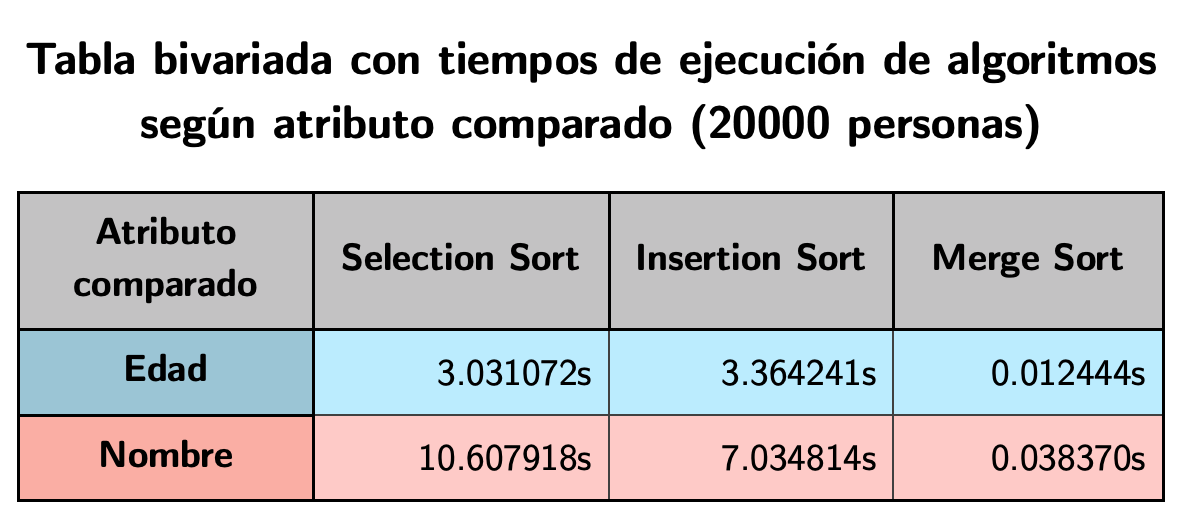
\includegraphics[scale = 0.465]{TABLA_BIVARIADA}\par
    \end{center}
\end{figure}

\begin{figure}[h]
    \begin{center}
        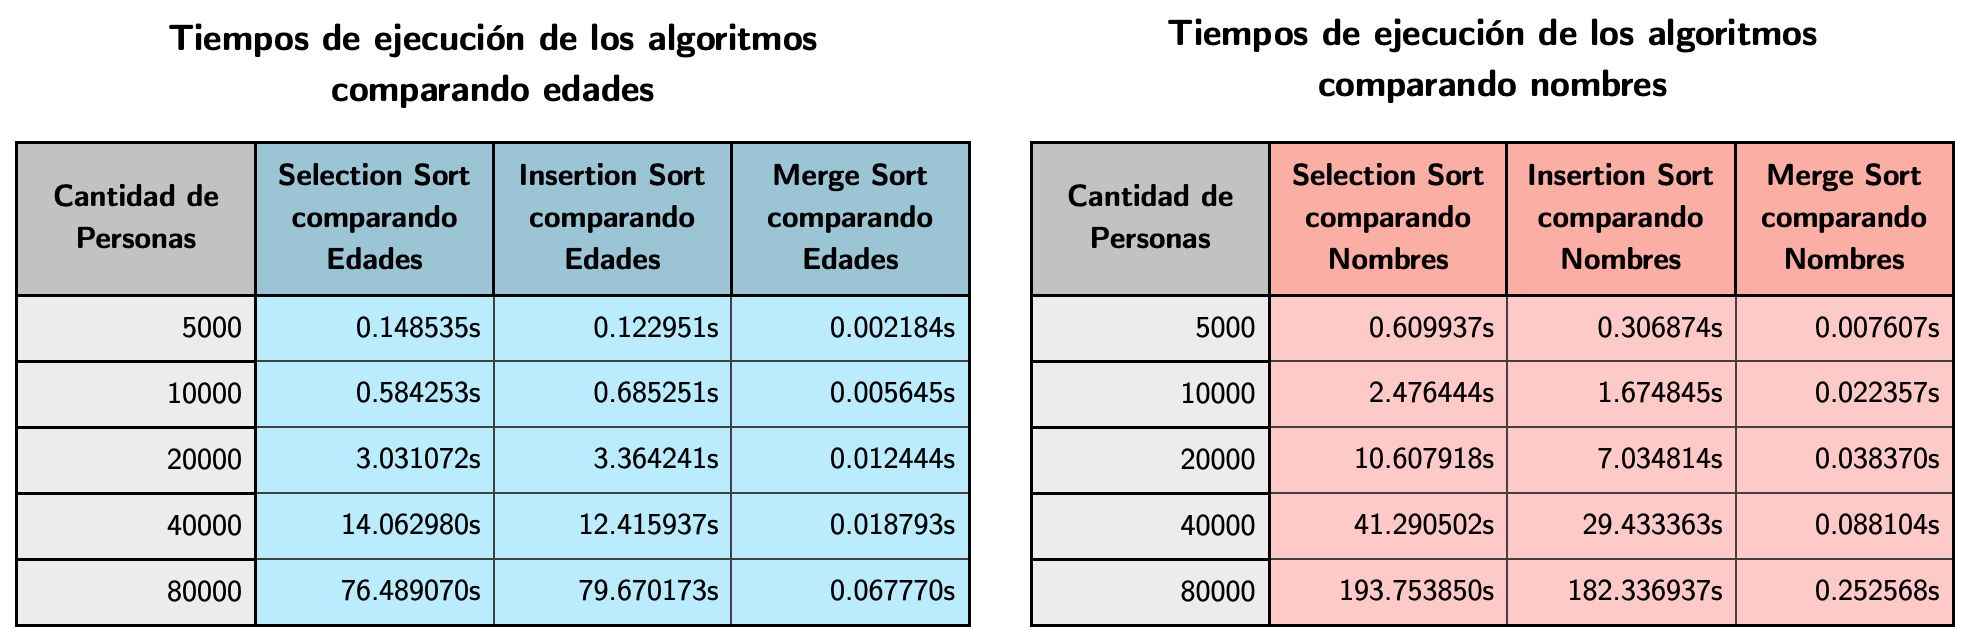
\includegraphics[scale = 0.5]{TABLAS}\par
    \end{center}
\end{figure}

Analizando los datos, se tiene que Selection Sort es el algoritmo con el mayor tiempo de ejecución, seguido de Insertion Sort y por último, con un tiempo considerablemente menor, Merge Sort. Estos tiempos reflejan el hecho de que Selection Sort recorre los elementos de la lista la misma cantidad de veces independientemente del orden inicial de la lista (es decir, el mejor y peor caso son iguales), y, en contraposición, la cantidad de operaciones que realiza Insertion Sort puede ser menor según el orden inicial de la lista. Por otro lado, como Merge Sort es una función recursiva y por tanto su ejecución requiere de una mayor cantidad de memoria que los otros dos algoritmos, la cantidad de operaciones que realiza (y consecuentemente el tiempo de ejecución) es mucho menor.\par

Como acotación, es relevante destacar que los tiempos en general de los algoritmos cuando comparan nombres son mayores a cuando comparan edades debido a que la función \verb|comp_nombres| realiza una mayor cantidad de operaciones que \verb|comp_edades|, lo que se refleja en mayor tiempo de ejecución con cantidades grandes.\par



\section{Bibliografía}
\begin{itemize}
    \item \verb|https://en.wikipedia.org/wiki/Insertion_sort|
    \item \verb|https://en.wikipedia.org/wiki/Selection_sort|
    \item \verb|https://en.wikipedia.org/wiki/Merge_sort|
    \item \verb|https://www.tutorialspoint.com/c_standard_library/c_function_clock.htm|
    \item \verb|https://theasciicode.com.ar|
\end{itemize}



\end{document}
